\chapter{Implementation}
%This chapter will describe how the implementation for the evaluation has been made. first lets take a look at what has to be implemented and why.
%\begin{itemize}
%\item Test Level\\
%this is the 3D environment that will be used to test the different control schemes. 
%\item Gyroscopic controls\\
%The control scheme that will use the gyroscope found in many mobile devices, what the gyroscope will be used for is to make it seem natural to turn around when looking in a virtual 3D space environment. 
%\item Joystick controls\\
%this control scheme is composed of two joystick like buttons, that respond to being dragged, one joystick will control the camera movement and the other the orientation of the camera. The idea is that this control scheme will seem familiar%reference to UX section
%to users because the common place console controller uses the same kind of dragable joystick.
%\item Standard button controls\\
%Because the previously described control schemes uses concepts that might not be immediately familiar to all users, this standard button control scheme was designed to see if users who are not familiar with joysticks and using their body movements, would perform better with a control scheme made out of buttons, all the buttons are able to trigger when being held down.
%\end{itemize}
%these four things are what is needed in the projects implementation. To implement this what is needed is some sort of framework for working within a 3D environment, there are two ways to go about this, either build such a framework from scratch or use one of the many game engines available. Since developing a fully fletched 3d engine is beyond the scope of this project, the choice fell on developing from within an available 3D engine

\subsection{Development of 3D elements}
Actual implementation consisted of creating level areas, 3D prefabs - cones and poles with string, sprites - notes and arrows. 3D elements were created using software "Maya" and textures with "Photoshop". Each level started by simple creation of a square representing a room. Then considerations of what test it will include were done and assets that were created were placed making different challenges. Picture \ref{3dDevelopment1} shows 3D cone and it's texture.
\begin{figure}[H]
\centering
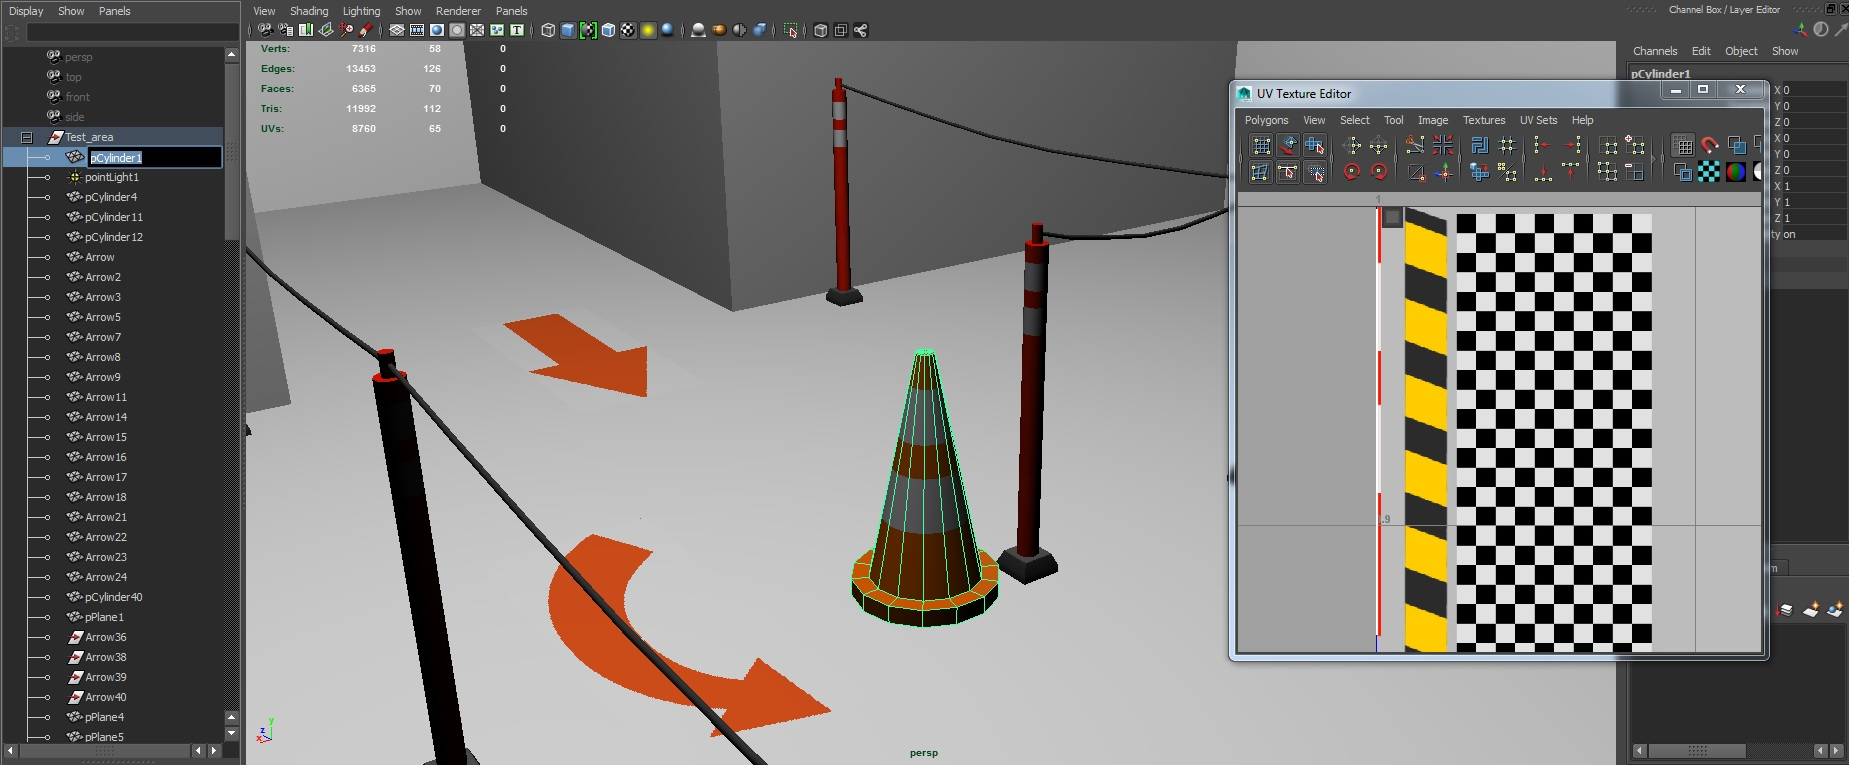
\includegraphics[scale=0.35]{3D_dev_7.jpg}
\caption{Picture of a cone from testing level}
\label {3dDevelopment1}
\end{figure}
Every object that required texturing, also needed its own UV map. UV map is 3 dimensional model representation in 2 dimensions - it helps to see and paint texture using tools as Photoshop. Following picture shows UV map as red lines, that helps to see the boundaries for the texturing in Photoshop \ref{3dDevelopment2}.
\begin{figure}[H]
\centering
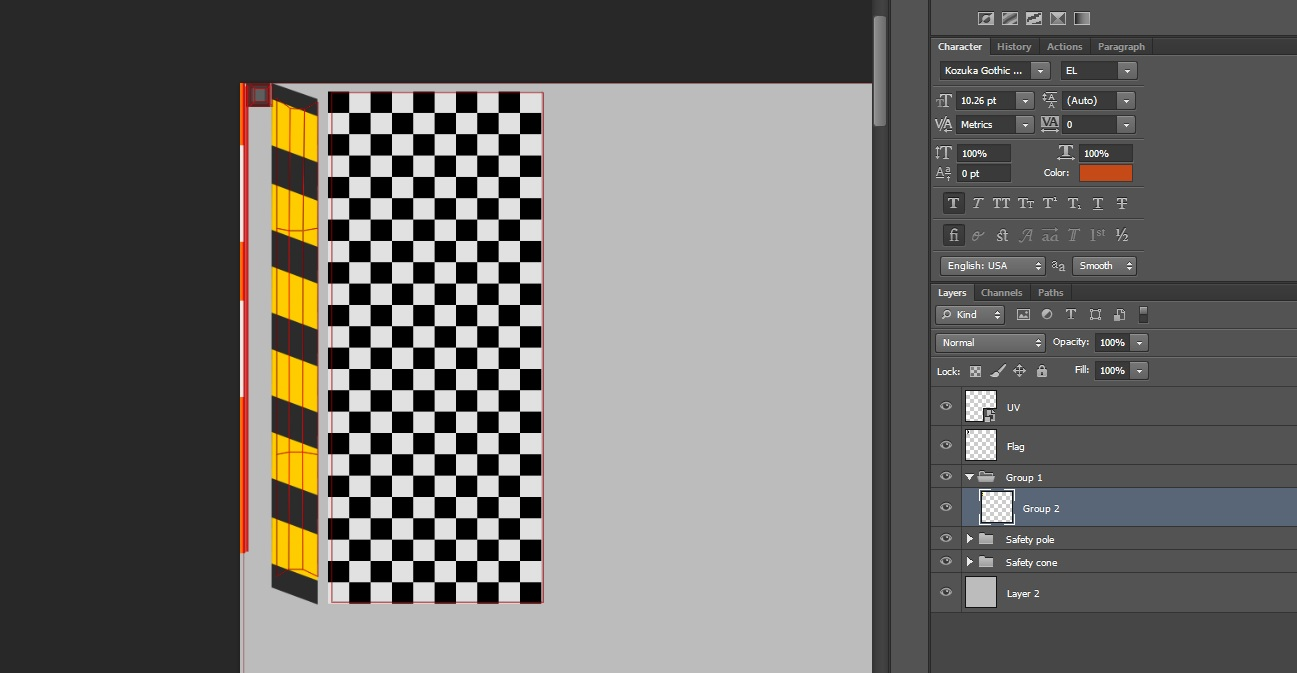
\includegraphics[scale=0.35]{3D_dev_8.jpg}
\caption{picture of a cone from testing level}
\label {3dDevelopment2}
\end{figure}
Text, directional arrows, and other symbols needed to be transparent so it would blend well with most of backgrounds. Such images were exported as png picture format to keep transparency \ref {3dDevelopment3}. 
\begin{figure}[H]
\centering

\includegraphics[scale=0.3]{3D_dev_9.png}
\caption{Pictures of elements that required transparency for game engine - also called sprites}
\label {3dDevelopment3}
\end{figure}
Since graphics and aesthetics were not focus of this test level, textures were created very minimalistic - without any shadowing, noise, imitation of being old or used etc. It also helped to make test very optimized in hardware performance, since textures size on disk were as little as few kilobytes.
\subsection{Unity Introduction}
For this implementation the choice was made to use the freely available Unity3D engine, this was chosen as Unity provides a lot of features that would otherwise mean that this project would not be possible to complete in the amount of time given. This section will provide a quick glance at what Unity is and introduce some common terms used within Unity. Everything that is seen in a Unity game is composed of {\tt GameObjects} these objects are what the scripts described in the following sections will be attached to. A newly created {\tt GameObject} will only contain what is known as a {\tt Transform} the transform is an object that holds the information about where the object is within the 3D space. It also holds the objects rotational information  and its scale.
the position of the object is expressed as a vector, a vector is a mathematical tool for representing a coordinate in space. As such vectors are the primarily tool that is used in unity for expressing things like velocity, position, forces etc.
\subsection{Buttons}
The buttons used in all three schemes are all created using unity's UI system. A button in the UI system is just a empty {\tt GameObject} that holds the following components:
\begin{itemize}
\item {\tt Rect Transform}\\
this component is equivalent to the regular {\tt Transform}.  However this component does not contain any information about the objects position in 3D space as it is part of the UI it only needs to know its coordinates on a 2D plane. The UI system provides a convenient way of making sure that UI will look the same no matter what screen size is used. It does this by having coordinates relative to a anchor point that is set by the developer. 
\item {\tt Button}\\
this is the standard script that unity uses to detect clicks on a button and can call methods on different objects when clicked. This script is the script that has been modified to allow for pressing and holding.
\item {\tt Image} \\
this component is a component that will draw an image on the canvas this image will be the full size of the button
\item 
\end{itemize}
\subsubsection{{\tt ButtonScript}}
{\tt ButtonScript} inherits from the in-built Unity {\tt Button} object. This is done so that the script can access the method {\tt   protected bool IsPressed()}. This script is the script that all buttons in both the buttons and gyro scene uses. it is a simple extension as all it has to do is check if the button is being pressed, and if it is then check which button it is and act accordingly. 
\subsection{Buttons Scene}
the button scene is the only scene that only uses  {\tt CamMovement} and {\tt ButtonScript} and as such is the simplest scene technically. Presented below is  the methods contained within {\tt camMovement}: 
\begin{itemize}
\item {\tt public void move(bool rightButton)}\\
this method will depending on the boolean given to it move the camera forward or backward. This is done by creating a directional vector formed from the transforms forward vector:
\begin{verbatim}
Vector3 directionVector = new Vector3(transform.forward.x, 
                                      0,
                                      transform.forward.z)
\end{verbatim}
the directional vector will always have a y component of 0 as the camera should not be able to move in the y direction. This vector is then multiplied by a integer variable that will take the value of either -1 or 1 depending on the value of {\tt rightButton} by converting the boolean into an integer with the line:\\
{\tt int goingForward = rightButton ? -1 : 1;}\\
Finally the directional vector is multiplied with a variable for determining the speed of the movement. This directional vector is then set as the velocity of the rigidbody that is attached to the GameObject. 

\item {\tt public void rotateLeftRight(bool right)}\\
this method will rotate the camera left or right in a similar manner to {\tt move} but where {\tt move} does not to anything to its y component the {\tt rotateLeftRight} method will only rotate in its y component an keep the rotation of the x component. This method uses {Quaternion.euler } to convert our euler angles into Quaternions, and {\tt Quaternion.Slerp} to smoothly make the camera rotate. This can be seen in figure \ref{Slerping} 
\begin{figure}[H]
\centering
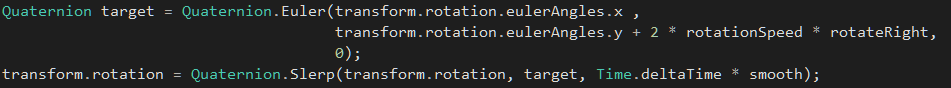
\includegraphics[scale=0.8]{Slerping.PNG}
\caption{conversion of quaternions into euler angles and use of the slerp function}
\label{Slerping}
\end{figure}
\item {\tt public void rotateUpDown(bool down)}\\
this function is more or less the exact same as {\tt rotateLeftRight} but where {\tt rotateLeftRight} makes changes to the y component of the rotation , {\tt rotateUpDown} rotates the x component. 

\item {\tt public void stopMovement()}\\
this function is a simple function to make all movement on the camera stop, it will set both the linear and angular velocity of the object to zero.
\end{itemize}


\subsection{Gyroscope Camera}
the gyroscopic camera uses two scripts to work, first and most importantly the {\tt GyroController} which is the script responsible for getting the input from the gyroscope and 
rotating accordingly. Unity can take input from the gyroscope directly, but if an object is rotated by the raw data from the gyroscope there will immediately be a problem as the coordinate system that is used to by gyroscope is a right-handed coordinate system 
\begin{figure}[H]
\centering
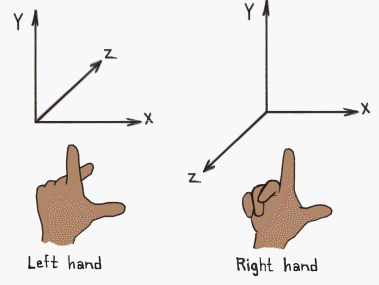
\includegraphics[scale=0.8]{left_right_hand.png}
\caption{right-handed vs left-handed coordinate systems}
\end{figure}
where unity uses a left hand coordinate system. To have the coordinates given by the gyroscope match the coordinates of Unity the {\tt GyroController} has a method for converting from right-handed to left-handed coordinate systems this method uses Quaternions which is how Unity handles rotation internally explaining quaternions is beyond the scope of this project\label{quaternions}
besides the {\tt GyroController}, this scene also uses the {\tt CamMovement} and {\tt ButtonScript} explained in the previous section, however in this scene only the forward and backward buttons are used, as the gyro is handling rotation of the camera.
\subsection{Joystick Scene} 
The joystick scene is technically the most difficult as this involves 
The joystick scene uses some of Unitys standard assets, these include:
\subsubsection*{Mobile Joystick}
The mobile joystick script creates two axis for unity's input manager. These two axis are then accessed by the first person controller and use these values to move camera. 


\subsubsection*{The Character controller}
this is actually a fully fleshed component, along with components like the transform, renderer etc. For this scene it is primarily used to generate a collider for the camera. 
\subsubsection*{First Person Controller}
Unity provides a standard first person controller that comes with a whole range of features. For this scene the FPS controller needs to take input from the joysticks, to do this the FPS controller's {\tt RotateView()} method has been modified to take input from the virtual axis created by the mobile joystick:
\begin{figure}[H]
\centering
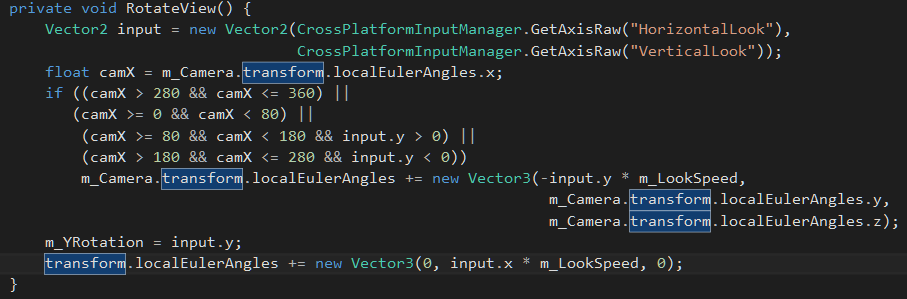
\includegraphics[scale=0.9]{RotateViewFunction.PNG}
\caption{the modified {\tt RotateView()} from the FPS controller}
\end{figure}
this method first reads the input from the axis named {\tt HorizontalLook} and {\tt VerticalLook} and stores these two values in a vector. This vector is essentially the directional vector we want to add to the cameras rotation. while a solution such as:
\begin{verbatim}
Vector3 dVector = new Vector3(input.x,input.y,0);
transform.localEulerAngles += dVector;
\end{verbatim} will make the transform rotate in the direction of the vector, it will also cause the camera angles to get stuck. This problem is known as gimbal locking, which is the situation where two rotational axis is pointing in the same direction. To avoid this problem the script checks to make sure that the camera is not rotated into a gimbal lock and adds the rotation to the cameras local rotation. The script does this by checking if the user is looking down or up at an angle of less than 80 degrees. 



